\documentclass[border=5mm]{standalone}
\usepackage{tikz}
\usetikzlibrary{positioning, arrows.meta, calc}
\usepackage{amsmath}

\begin{document}
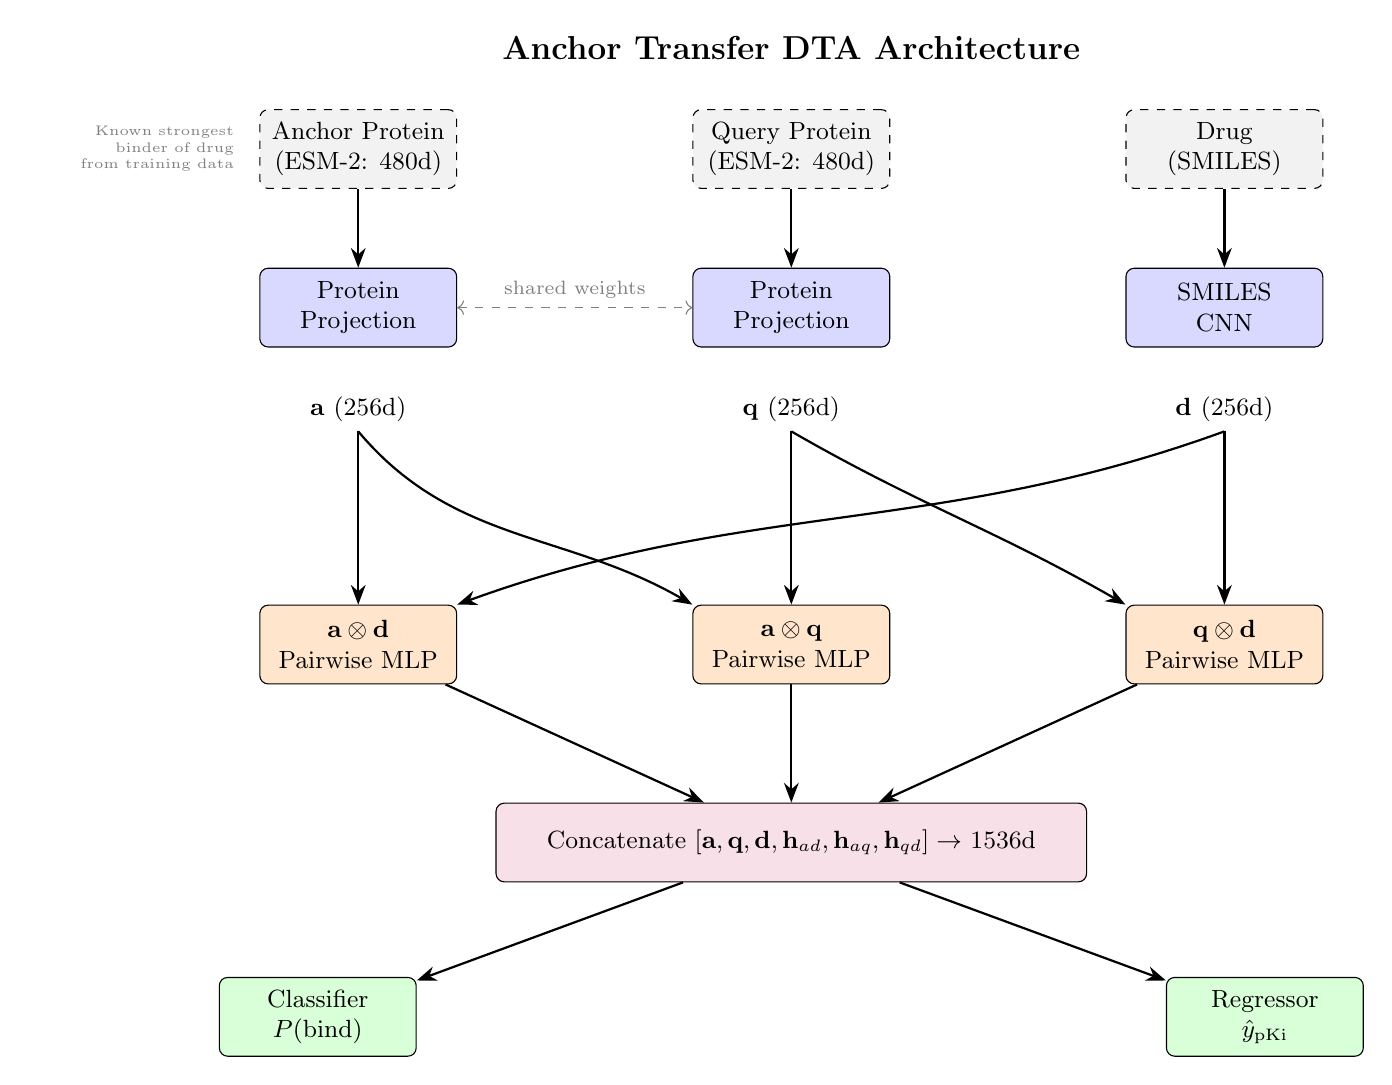
\begin{tikzpicture}[
    node distance=1.4cm and 3cm,
    block/.style={rectangle, draw, rounded corners=3pt, minimum height=1cm, minimum width=2.5cm, align=center, font=\small},
    encoder/.style={block, fill=blue!15},
    interaction/.style={block, fill=orange!20},
    head/.style={block, fill=green!15},
    input/.style={block, fill=gray!10, dashed},
    arrow/.style={-{Stealth[length=2.5mm]}, thick},
    crossarrow/.style={-{Stealth[length=2.5mm]}, thick},
]

% Title
\node[font=\large\bfseries] (title) {Anchor Transfer DTA Architecture};

% Inputs (wider spacing)
\node[input, below=0.5cm of title, xshift=-5.5cm] (anchor) {Anchor Protein\\(ESM-2: 480d)};
\node[input, below=0.5cm of title] (query) {Query Protein\\(ESM-2: 480d)};
\node[input, below=0.5cm of title, xshift=5.5cm] (drug) {Drug\\(SMILES)};

% Encoders
\node[encoder, below=1cm of anchor] (aproj) {Protein\\Projection};
\node[encoder, below=1cm of query] (qproj) {Protein\\Projection};
\node[encoder, below=1cm of drug] (denc) {SMILES\\CNN};

% Shared weights annotation
\draw[dashed, gray, <->] (aproj.east) -- node[above, font=\scriptsize, gray] {shared weights} (qproj.west);

% Embedding labels
\node[below=0.5cm of aproj, font=\small\itshape] (alabel) {$\mathbf{a}$ \normalfont(256d)};
\node[below=0.5cm of qproj, font=\small\itshape] (qlabel) {$\mathbf{q}$ \normalfont(256d)};
\node[below=0.5cm of denc, font=\small\itshape] (dlabel) {$\mathbf{d}$ \normalfont(256d)};

% Pairwise interaction MLPs — repositioned logically
\node[interaction, below=2.2cm of alabel] (pw_ad) {$\mathbf{a} \otimes \mathbf{d}$\\Pairwise MLP};
\node[interaction, below=2.2cm of qlabel] (pw_aq) {$\mathbf{a} \otimes \mathbf{q}$\\Pairwise MLP};
\node[interaction, below=2.2cm of dlabel] (pw_qd) {$\mathbf{q} \otimes \mathbf{d}$\\Pairwise MLP};

% Fusion
\node[block, fill=purple!12, below=1.5cm of pw_aq, minimum width=7.5cm] (fusion)
    {Concatenate $[\mathbf{a}, \mathbf{q}, \mathbf{d}, \mathbf{h}_{ad}, \mathbf{h}_{aq}, \mathbf{h}_{qd}] \rightarrow$ 1536d};

% Prediction heads
\node[head, below left=1.2cm and 1cm of fusion] (cls) {Classifier\\$P(\text{bind})$};
\node[head, below right=1.2cm and 1cm of fusion] (reg) {Regressor\\$\hat{y}_{\text{pKi}}$};

%% === Arrows ===

% Inputs to encoders (straight down)
\draw[arrow] (anchor) -- (aproj);
\draw[arrow] (query) -- (qproj);
\draw[arrow] (drug) -- (denc);

% --- Direct connections (straight down, no crossing) ---
\draw[arrow] (alabel) -- (pw_ad);   % a → a⊗d
\draw[arrow] (qlabel) -- (pw_aq);   % q → a⊗q
\draw[arrow] (dlabel) -- (pw_qd);   % d → q⊗d

% --- Short cross-connections (gentle curves) ---
% a → a⊗q : left to center
\draw[arrow] (alabel.south) to[out=-50, in=150] (pw_aq.north west);
% q → q⊗d : center to right
\draw[arrow] (qlabel.south) to[out=-30, in=150] (pw_qd.north west);

% --- Long cross-connection (wide curve, goes below the short curves) ---
% d → a⊗d : right to left
\draw[crossarrow] (dlabel.south) to[out=-160, in=20] (pw_ad.north east);

% Pairwise MLPs to fusion
\draw[arrow] (pw_ad) -- (fusion);
\draw[arrow] (pw_aq) -- (fusion);
\draw[arrow] (pw_qd) -- (fusion);

% Fusion to heads
\draw[arrow] (fusion) -- (cls);
\draw[arrow] (fusion) -- (reg);

% Annotation: anchor selection
\node[left=0.2cm of anchor, font=\tiny, text width=2.5cm, align=right, gray] {Known strongest\\binder of drug\\from training data};

\end{tikzpicture}
\end{document}
